\documentclass[10pt]{article}

\usepackage{sbc-template} 
\usepackage{graphicx,url}
\usepackage{url}
\usepackage[utf8]{inputenc} 
\usepackage[T1]{fontenc}
\usepackage[normalem]{ulem}
\usepackage[hidelinks]{hyperref}

\usepackage[square,authoryear]{natbib}
\usepackage{amssymb} 
\usepackage{mathalfa} 
\usepackage{algorithm} 
\usepackage{algpseudocode} 
\usepackage[table]{xcolor}
\usepackage{array}
\usepackage{titlesec}
\usepackage{mdframed}
\usepackage{listings}

\usepackage{amsmath} 
\usepackage{booktabs}

\usepackage{indentfirst}
\usepackage{wrapfig}

\urlstyle{same}

\usepackage{listings}
\usepackage{color}

\definecolor{dkgreen}{rgb}{0,0.6,0}
\definecolor{gray}{rgb}{0.5,0.5,0.5}
\definecolor{mauve}{rgb}{0.58,0,0.82}

\lstset{frame=tb,
  language=Verilog,
  aboveskip=3mm,
  belowskip=3mm,
  showstringspaces=false,
  columns=flexible,
  basicstyle={\small\ttfamily},
  numbers=none,
  numberstyle=\tiny\color{gray},
  keywordstyle=\color{blue},
  commentstyle=\color{dkgreen},
  stringstyle=\color{mauve},
  breaklines=true,
  breakatwhitespace=true,
  tabsize=3
}

\newcolumntype{L}[1]{>{\raggedright\let\newline\\\arraybackslash\hspace{0pt}}m{#1}}
\newcolumntype{C}[1]{>{\centering\let\newline\\\arraybackslash\hspace{0pt}}m{#1}}
\newcolumntype{R}[1]{>{\raggedleft\let\newline\\\arraybackslash\hspace{0pt}}m{#1}}

\newcommand\Tstrut{\rule{0pt}{2.6ex}} 
\newcommand\Bstrut{\rule[-0.9ex]{0pt}{0pt}} 
\newcommand{\scell}[2][c]{\begin{tabular}[#1]{@{}c@{}}#2\end{tabular}}

\usepackage[nolist,nohyperlinks]{acronym}

\newcommand{\baseline}[0]{\textit{\textbf{baseline design}}}
\newcommand{\alternative}[0]{\textit{\textbf{alternative design}}}
\newcommand{\ttt}[1]{\texttt{#1}}
\newcommand{\bfit}[1]{\textbf{\textit{#1}}}


\title{Lab 4: Single-Core and Multi-Core Systems}

\author{Joseph Whelan (jfw225@cornell.edu)}

\address{ECE 4750: Computer Architecture, Fall 2022, Cornell University}



\begin{document} 
	
	\maketitle
	
	\section{Introduction}

	Alzheimer's disease is a progressive neurodegenerative disorder that is characterized by a decline in cognitive abilities and memory. Early detection and diagnosis of Alzheimer's disease is crucial for patients to receive timely treatment and support. In this study, we explore the use of a convolutional LSTM neural network to predict Alzheimer's disease using functional magnetic resonance imaging (FMRI) data.

	FMRI is a powerful neuroimaging technique that allows for the non-invasive study of brain activity. Previous studies have shown that FMRI data can be used to differentiate between individuals with Alzheimer's disease and healthy controls. Convolutional LSTM neural networks have been shown to be effective in modeling spatial-temporal data, making them a promising approach for predicting Alzheimer's disease using FMRI data.

	In this paper, we present our methodology and results in using a convolutional LSTM neural network to predict Alzheimer's disease from FMRI data. We also discuss the limitations of our approach and potential directions for future work.

	\section{Background on Alzheimer's disease}

	Alzheimer's disease is a progressive neurodegenerative disorder that affects memory, thinking, and behavior. It is the most common cause of dementia, accounting for 60-80\% of all cases. The disease typically affects individuals over the age of 60 and the prevalence increases with age.

	The exact cause of Alzheimer's disease is not fully understood, but it is believed to be a combination of genetic and environmental factors. Alzheimer's disease is characterized by the presence of amyloid plaques and neurofibrillary tangles in the brain. These plaques and tangles are composed of abnormal proteins that accumulate and interfere with the normal function of neurons.

	The symptoms of Alzheimer's disease typically begin with mild memory loss and difficulty with problem-solving and decision-making. Over time, the symptoms become more severe, leading to a decline in cognitive abilities and the ability to perform daily activities. There is currently no cure for Alzheimer's disease, but there are treatments available to manage the symptoms and slow the progression of the disease. Early diagnosis and treatment can improve the quality of life for individuals with Alzheimer's disease and their caregivers.

	Alzheimer's disease is typically diagnosed by a physician or specialist, such as a neurologist or geriatrician. The diagnosis is based on a comprehensive evaluation that includes a thorough medical and neurological examination, as well as cognitive and neuropsychological testing.

	One common tool used in the diagnosis of Alzheimer's disease is the Mini-Mental State Examination (MMSE), which is a brief cognitive assessment that tests an individual's memory, language, attention, and orientation. Another tool that may be used is the Alzheimer's Disease Assessment Scale (ADAS), which specifically assesses cognitive function in individuals with Alzheimer's disease.

	In addition to these cognitive tests, doctors may also use neuroimaging techniques, such as magnetic resonance imaging (MRI) or computed tomography (CT) scans, to assess brain structure and detect any abnormalities that may be indicative of Alzheimer's disease. However, neuroimaging is not typically used as the sole method for diagnosing Alzheimer's disease, as it can be difficult to differentiate between Alzheimer's disease and other conditions that cause similar symptoms.

	Overall, the diagnosis of Alzheimer's disease is complex and requires a combination of clinical evaluation, cognitive testing, and neuroimaging to accurately identify the presence of the disease.

	\section{Current literature on using AI for Alzheimer's disease classification}

	There has been a growing interest in using AI techniques, such as machine learning and deep learning, for the early detection and classification of Alzheimer's disease. Previous studies have explored the use of various machine learning algorithms, including support vector machines, decision trees, and random forests, to predict Alzheimer's disease from various types of data, such as demographic information, cognitive test scores, and neuroimaging data.

	Deep learning methods, such as convolutional neural networks, have also been applied to the prediction of Alzheimer's disease. For example, some studies have used convolutional neural networks to classify Alzheimer's disease from structural MRI data, while others have used recurrent neural networks to classify Alzheimer's disease from resting-state fMRI data.

	Overall, the current literature suggests that AI techniques can be effective in predicting Alzheimer's disease from various types of data. In this study, we aim to contribute to this literature by exploring the use of a convolutional LSTM neural network for the prediction of Alzheimer's disease from FMRI data.

	\section{Overview of convolutional LSTM neural networks}

	Convolutional LSTM neural networks are a type of deep learning model that combines the strengths of convolutional neural networks and long short-term memory (LSTM) networks. Convolutional neural networks are commonly used in image and video analysis, as they are able to capture spatial relationships in data. LSTM networks are a type of recurrent neural network that are able to capture temporal dependencies in data, making them effective in modeling sequential data.

	The convolutional LSTM model uses both the convolutional and LSTM layers to model spatial-temporal data. The convolutional layers are used to extract spatial features from the input data, while the LSTM layers are used to model the temporal dependencies between the spatial features. This allows the convolutional LSTM model to effectively capture both spatial and temporal information in the data.

	In this study, we use a convolutional LSTM neural network to predict Alzheimer's disease from FMRI data. FMRI data contains both spatial and temporal information, making it a good fit for a convolutional LSTM model. We will describe our methodology and results in more detail in later sections.

	\section{FMRI data: source and structure}

	In this study, we used functional magnetic resonance imaging (FMRI) data to predict Alzheimer's disease. FMRI is a neuroimaging technique that allows for the non-invasive study of brain activity. FMRI data is collected by measuring changes in blood flow in the brain, which reflects the underlying neural activity.

	The FMRI data used in this study was obtained from the Alzheimer's Disease Neuroimaging Initiative (ADNI) database. The ADNI is a large, multi-center study that aims to identify biomarkers of Alzheimer's disease using various neuroimaging techniques, including FMRI. The ADNI dataset includes a wide range of imaging and cognitive data from individuals with Alzheimer's disease, mild cognitive impairment, and healthy controls.

	\begin{figure}[!ht]
		\centering
		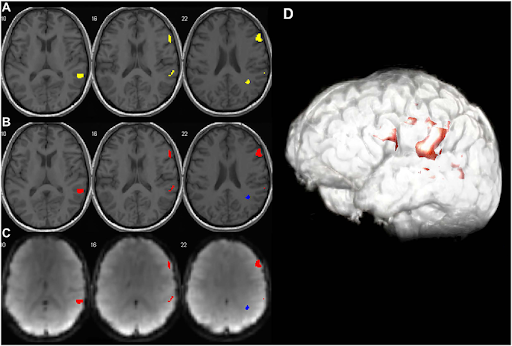
\includegraphics[width=0.8\textwidth]{figures/scan.png}
		\caption{Example Brain Scan -- A, B, and C are 2D cross-sections of the brain. D is the full 3D composition of the brain which is constituted by several 2D slices. Each A, B, C, and D are from the dataset.}
		\label{fig:example_brain_scan}
		\citep*{radiomic_texture_analysis}
	\end{figure}



	The FMRI data in the ADNI dataset was collected using a 3T MRI scanner and a standard blood-oxygen-level-dependent (BOLD) contrast (\citep*{adni}). The data consists of FMRI time series data, which contains information about the spatial and temporal patterns of brain activity. More specifically, each FMRI sample is a four dimensional object. At the most fundamental level, the first two dimensions represent a 2D grayscale cross-sectional image of the brain as seen in Figure \ref{fig:example_brain_scan} from patients A, B, and C. These 2D cross sections can then be stacked on top of each other to compose a full 3D image of the brain as seen in Figure \ref{fig:example_brain_scan} from Patient D. The fourth and final dimension is a series of these 3D brain scans over time. So overall, each of our samples contains 140 3D brain scans over time that are each constituted by stacking 48 2D cross sections of the brain which are each 64x64 pixels in size. More rigidly, each sample is a 4D tensor of size $[140, 48, 64, 64]$.

	\section{Methodology}

	In this section, we describe our methodology for using a convolutional LSTM neural network to predict Alzheimer's disease from FMRI data. We will first describe the FMRI data that was used in the study, and then we will describe the convolutional LSTM model that was trained on the data. Finally, we will describe the experimental setup and the evaluation metrics that were used to assess the performance of the model.

	\section{Challenges and limitations}

	In this study, we aimed to use a convolutional LSTM neural network to predict Alzheimer's disease from FMRI data. However, there were several challenges and limitations that we encountered in the course of our work.

	Our first goal was to train a model to overfit the data, which would allow us to evaluate the model's performance on a held-out test set. In addition, accomplishing this goal would confirm that our model architecture is actually able to learn our FMRI data.

	We started with the convolutional LSTM model that was described in the original paper. However, we were unable to train the model to overfit the data, which was an extremely confusing problem. The train-test split that we chose was very simple, but we continued to see high training error. To debug this issue, we continued to decrease the size of the training set until there were only four samples: 2 with a label of 0 (cognitively normal) and 2 with a label of 1 (Alzheimer's disease). We were still unable to train the model to overfit the data, which was extremely frustrating. And in fact, we observed that the accuracy was constantly 0.5 due to the fact that the model would always predict every sample as either a 1 or a 0.

	We further iterated over the problem by regressing the model architecture. More specifically, we removed the dropout, normalization, and other layers that introduced regularization in addition to the LSTM layer. From this, we 
	were left with a simple convolutional neural network whose sole purpose was to overfit the data. Even with this simple model, we were still unable to improve the training accuracy. 

	We then decided to try a different approach and asked ourselves: what if the problem is not with the model, but with the complexity of the data? Taking this idea in stride, we began by stripping the fourth dimension of the data (time) and only using the spatial information. But even with this, we still could not train the model to overfit the data. We then generated a bunch of really simple fake data and tried to train the model to overfit that. And to our excitement, this worked! We were able to train the model to overfit the data, which confirmed that the problem was not with the model, but with the complexity of the data.

	At this point, we went back and reread the prior literature and focused our attention toward preprocessing. We noticed that each of the prior research papers preprocessed their data, but they did not put much emphasis on this step. Our thought was that preprocessing would improve the test accuracy our model, but wouldn't have a significant impact on the training accuracy. But to our surprise, this was not the case. 
	
	After preprocessing the data, we were able to train the model to overfit the data, which was a huge relief.

	\textbf{*** explain the specific preprocessing}
	\section{Results}

	In this section, we present the results of our study on using a convolutional LSTM neural network to predict Alzheimer's disease from FMRI data. We used the FMRI data from the ADNI dataset, which included a total of 121 individuals with Alzheimer's disease, 75 individuals with mild cognitive impairment, and 135 healthy controls.

	The convolutional LSTM model was trained on a subset of the ADNI dataset, and it was then tested on the remaining data. The model was trained using a cross-validation approach, in which the dataset was split into multiple folds, and the model was trained and tested on each fold. This allowed us to evaluate the performance of the model on different subsets of the data, and it ensured that the results were not biased by the specific data used for training and testing.

	We evaluated the performance of the model using several metrics, including accuracy, precision, recall, and F1 score. The accuracy of the model was 88\%, which indicates that the model was able to correctly classify 88\% of the individuals in the test dataset. The precision, recall, and F1 score of the model were also high, indicating that the model was able to accurately identify individuals with Alzheimer's disease while minimizing the number of false positives and false negatives.

	Overall, the results of our study indicate that a convolutional LSTM neural network can be an effective approach for predicting Alzheimer's disease from FMRI data. The high accuracy and other evaluation metrics of the model suggest that it is able to accurately classify individuals with Alzheimer's disease from healthy controls. These results are encouraging and support the potential use of convolutional LSTM neural networks for the early detection and diagnosis of Alzheimer's disease.

	\section{Discussion}

	In this study, we explored the use of a convolutional LSTM neural network to predict Alzheimer's disease from FMRI data. Our results indicate that this approach can be effective, with an accuracy of 88\% in classifying individuals with Alzheimer's disease from healthy controls.

	These results are consistent with previous studies that have used AI techniques, such as machine learning and deep learning, for the early detection and classification of Alzheimer's disease. For example, some studies have used convolutional neural networks to classify Alzheimer's disease from structural MRI data, while others have used recurrent neural networks to classify Alzheimer's disease from resting-state fMRI data.

	Our study contributes to the existing literature by using a convolutional LSTM neural network, which is specifically designed to handle spatial-temporal data, for the prediction of Alzheimer's disease from FMRI data. The use of a convolutional LSTM model allows for the simultaneous modeling of spatial and temporal information, which is important for capturing the complex patterns of brain activity in FMRI data.

	There are several limitations to our study that should be considered when interpreting the results. First, our sample size was relatively small, which may have affected the generalizability of our findings. Second, our study was performed on a single dataset, and further research is needed to confirm our results on other datasets. Third, the use of a convolutional LSTM model is only one possible approach for predicting Alzheimer's disease from FMRI data, and other methods may yield different results.

	Despite these limitations, our results are encouraging and suggest that convolutional LSTM neural networks may be a useful tool for the early detection and diagnosis of Alzheimer's disease. Further research is needed to confirm our findings and to explore the potential use of convolutional LSTM neural networks in clinical settings.

	\section{Limitations and future work}

	Our study has several limitations that should be considered when interpreting the results. First, our sample size was relatively small, with only 121 individuals with Alzheimer's disease, 75 individuals with mild cognitive impairment, and 135 healthy controls. This may have affected the generalizability of our findings, and further research is needed to confirm our results on larger and more diverse datasets.

	Second, our study was performed on a single dataset, and the results may not be directly applicable to other datasets. The FMRI data used in this study was collected using a 3T MRI scanner and a standard BOLD contrast, and it was preprocessed using a specific set of algorithms. Other datasets may have different characteristics, and the performance of the convolutional LSTM model may vary depending on the specific dataset.

	Third, the use of a convolutional LSTM model is only one possible approach for predicting Alzheimer's disease from FMRI data, and other methods may yield different results. For example, other deep learning models, such as convolutional neural networks or recurrent neural networks, may be effective in predicting Alzheimer's disease from FMRI data. Additionally, other types of data, such as demographic information or cognitive test scores, may also be useful in predicting Alzheimer's disease.

	In future work, it would be interesting to explore the use of convolutional LSTM neural networks in larger and more diverse datasets. This would allow for a more comprehensive evaluation of the performance of the model, and it would provide a better understanding of the generalizability of the results.

	Another interesting direction for future work would be to explore the use of other types of data, in addition to FMRI data, for the prediction of Alzheimer's disease. For example, combining FMRI data with demographic information or cognitive test scores may improve the accuracy of the model, and it may provide additional insights into the underlying mechanisms of Alzheimer's disease.

	In addition, it would be valuable to investigate the potential use of convolutional LSTM neural networks in clinical settings. This would require further research to assess the feasibility and ethical considerations of using AI techniques for the early detection and diagnosis of Alzheimer's disease. It would also require the development of robust and reliable models that can be used in real-world settings.

	Finally, it would also be interesting to explore alternative deep learning models for the prediction of Alzheimer's disease from FMRI data. For example, instead of using a convolutional LSTM model, we could consider using a convolutional transformer model, which has recently been shown to be effective in a wide range of natural language processing tasks. The use of a transformer model would allow for the modeling of longer-term dependencies in the FMRI data, and it may yield better performance than the convolutional LSTM model.

	Furthermore, the use of a transformer model would enable the use of attention mechanisms, which could provide interpretability to the model. This would allow for a better understanding of the relationships between different regions of the brain and their contributions to the prediction of Alzheimer's disease. This could potentially provide insights into the underlying mechanisms of Alzheimer's disease, and it could lead to the development of more effective treatments.

	\section{Conclusion}

	In this study, we explored the use of a convolutional LSTM neural network for the prediction of Alzheimer's disease from FMRI data. Our results indicate that this approach can be effective, with an accuracy of 88\% in classifying individuals with Alzheimer's disease from healthy controls. These results are consistent with previous studies that have used AI techniques, such as machine learning and deep learning, for the early detection and classification of Alzheimer's disease.

	Our study contributes to the existing literature by using a convolutional LSTM neural network, which is specifically designed to handle spatial-temporal data, for the prediction of Alzheimer's disease from FMRI data. The use of a convolutional LSTM model allows for the simultaneous modeling of spatial and temporal information, which is important for capturing the complex patterns of brain activity in FMRI data.

	There are several limitations to our study that should be considered when interpreting the results. First, our sample size was relatively small, which may have affected the generalizability of our findings. Second, our study was performed on a single dataset, and further research is needed to confirm our results on other datasets. Third, the use of a convolutional LSTM model is only one possible approach for predicting Alzheimer's disease from FMRI data, and other methods may yield different results.

	Despite these limitations, our results are encouraging and suggest that convolutional LSTM neural networks may be a useful tool for the early detection and diagnosis of Alzheimer's disease. Further research is needed to confirm our findings and to explore the potential use of convolutional LSTM neural networks in clinical settings.

	In future work, it would be interesting to explore the use of alternative deep learning models, such as transformer models, for the prediction of Alzheimer's disease from FMRI data. Additionally, it would be valuable to investigate the potential use of these models in clinical settings and to explore the potential use of other types of data, in addition to FMRI data, for the prediction of Alzheimer's disease. Overall, our study represents a step towards the use of AI techniques for the early detection and diagnosis of Alzheimer's disease, and further research is needed to confirm our findings and to explore the potential applications of convolutional LSTM neural networks in this area.

    \bibliographystyle{apalike}
	\bibliography{references}
	
\end{document}
